\section{General algebra}
In the following sections, we will take care to differentiate between the definition of a concept (like of an inner product) and its implementation. The definition of an inner product is based on properties that a thing has to fulfill, whereas the implementation begins with a definition and is then followed by a proof that the properties hold under that definition.

We will mention the following implementations: the vectorspace of coordinate free oriented lengths, the vectorspace $\reals^n$, which is the same as oriented length but put inside of a coordinate system(euclidian or angular), the vectorspace of matrices, and $C_{[a,b]}$, the vectorspace of continuous functions.

\subsection{Vector spaces}
 

\begin{definition}[Vector space] A vector space $V$ is a set closed over two operations: scalar multiplication and vector addition. These two operations must fullfill the following properties:
\begin{itemize}
    \item $V$ is closed under scalar multiplication and vector-addition: $a\vec{v} \in V, \vec{v} + \vec{w} \in V$
    \item vector-addition is commutative: $\vec{v} + \vec{w} = \vec{w} + \vec{v}$
    \item vector-addition is associative: $(\vec{u} + \vec{v}) + \vec{w} = \vec{u} + (\vec{v} + \vec{w})$
    \item $\vec{0}$ is the additive identity: $\vec{v} + \vec{0} = \vec{v}$
    
    \item $a(b\vec{v}) = (ab)\vec{v}$
    \item Vector-addition and scalar-multiplication are distributive (part 1): $a(\vec{v} + \vec{w}) = a\vec{v} + a\vec{w}$
    \item Vector-addition and scalar-multiplication are distributive (part 2): $(a+b)\vec{v} = a\vec{v} + b\vec{v}$
\end{itemize}
\end{definition}

The most common vectorspaces are certainly $\reals^n$ and functionspaces.
The implementations of the above defined scalar product and vector addition are trivial.

\paragraph{Subspaces of vectorspaces}
A set $U$ is a subspace of a vectorspace $V$, iff $U \subset V$ and $U$ is a vectorspace.

\paragraph{linear independence} 
The elements in $A$, a subset of a vectorspace, are linearly independent iff $\forall \alpha_1, ...,\alpha_n: [( \sum \alpha_i \vec{a}_i = 0 ) \iff ( \alpha_1 = \alpha_2 = ... = 0 )]$. Note that this reduces automatically to $\forall \alpha_1, ...,\alpha_n: [\sum_i^n \alpha_i b_i = 0 \then (\alpha_1 = ... = \alpha_n = 0)]$, because the $\leftarrow$ case is always true. 

Consequently, linear dependence is defined as $B:ld \equiv \thereis \alpha_1, ..., \alpha_2: [(\alpha_1 \neq 0 \lor ... \lor \alpha_n \neq 0) \land ( \sum_i^n \alpha_i b_i = 0 )]$.


\begin{proof}
    Prove that iff $B:ld$, then one of the elements of $B$ is a linear combination of the others. 
\end{proof}


\paragraph{Bases}
A set $B$ is a base to a vectorspace $V$ iff $ B \subseteq V \land  \forall v \in V: \thereis ! \alpha_1, ..., \alpha_n : v = \sum_i \alpha_i b_i $. It is easy to prove that this means that
$ B:baseV \iff ( B:li \land B:spanV ) $. 



The dimension of a vecotrspace $S$ is defined as the size of its base $B$. That means to get a base for $\reals^2$, we never need more than two vectors. We'll prove this for the example of $S = \reals^2$:

\begin{proof} \label{proofBaseSizeEqualsSpaceDimension}
For any three vectors chosen from $\reals^2$, at least one must be a linear combination of the others. \\
    \subprf{$\vec{a}, \vec{b}, \vec{c} \in \reals^2$ }{ $\vec{a}:ld(\vec{b}, \vec{c}) \lor \vec{b}:ld(\vec{a}, \vec{c}) \lor \vec{c}:ld(\vec{a}, \vec{b})$ }{
        
        \subprf{Without loss of generality, assume $ \vec{a}:li(\vec{b}, \vec{c}) $ and $\vec{b}:li(\vec{a}, \vec{c})$}{$\vec{c}:ld(\vec{a}, \vec{b})$}{
        
            $\vec{a}$ and $\vec{b}$ form a base for $\reals^2$. That means any $\vec{x} \in \reals^2$ is a linear combination of these two ... including $\vec{c}$.
        
        }
    }
\end{proof}



\subsection{Inner product spaces}
Vector spaces don't define anything about lengths, angles or projections. This lack is alleviated by adding a inner product. 

\begin{definition}[Inner product space] The inner product is defined as any operation that has the following properties:
\begin{itemize}
    \item $(a\vec{u}) \innerprod \vec{v} = a (\vec{u} \innerprod \vec{v}) $
    \item $(\vec{u} + \vec{v}) \innerprod \vec{w} = \vec{u} \innerprod \vec{w} + \vec{v} \innerprod \vec{w}$
    \item $\vec{u} \innerprod \vec{v} = \vec{v} \innerprod \vec{u}$
    \item $\vec{v} \neq \vec{0} \then \vec{v} \innerprod \vec{v} > 0$
\end{itemize}
\end{definition}

In inner product spaces, we can define norms, orthogonality, and angles. 

As for norms:

$$ |\vec{v}|^2 = \vec{n} \innerprod \vec{n} $$

And orthogonality:

$$ \vec{v} \orth \vec{u} \iff \vec{v} \innerprod \vec{u} = 0$$

And finally angles: 

$$ cos\theta = \frac{\vec{v} \innerprod \vec{u}}{|\vec{v}||\vec{u}|}$$



As one nice little application, consider this statement. 
\begin{proof}
    \subprf{Suppose $|\vec{u}| = |\vec{v}|$.}{$\vec{u} + \vec{v} \orth \vec{u} - \vec{v}$}{
        This is to prove that $(\vec{u} + \vec{v}) \innerprod (\vec{u} - \vec{v}) = 0$ \\
        The above can be rewritten to $\vec{u} \innerprod \vec{u} - \vec{u} \innerprod \vec{v} + \vec{v} \innerprod \vec{u} - \vec{v} \innerprod \vec{v}$ \\
        The two middle terms cancel out, and the two outer terms equal $|\vec{u}|^2$ and $|\vec{v}|^2$, respectively. \\
        Usign the given, these terms are equal.
    }
\end{proof}

Other properties of the norm are also easily proved:

\begin{itemize}
    \item $|a\vec{v}| = |a||\vec{v}|$
    \item $|\vec{v} + \vec{w}| = |\vec{v}| + |\vec{w}|$
    \item $|\vec{v}| \geq 0$
    \item $|\vec{v}| = 0 \iff \vec{v} = \vec{0}$
\end{itemize}

Two more important statements that can be proven for the general inner product spaces are the pythagorean theorem and the Cauchy-Schwartz inequality. 

\begin{proof}
    Pythagorean theorem.\\
    \subprf{Suppose $\vec{u} \orth \vec{v}$.}{$|\vec{u}|^2 + |\vec{v}|^2 = |\vec{u} + \vec{v}|^2 $}{
    }
\end{proof}


\begin{proof}
    Cauchy-Schwartz inequality.\\
    \subprf{}{$|\vec{u}||\vec{v}| \geq |\vec{u} \innerprod \vec{v}| $}{
    }
\end{proof}


An implementation of this inner product in dimension-free oriented length-space would be:

$$\vec{v} \innerprod \vec{w} = |\vec{v}||\vec{w}|cos\theta$$

Based on this definition, the projection of $\vec{v}$ onto $\vec{u}$ is defined as: 

$$ P_{\vec{u}}(\vec{v}) = |\vec{v}| cos\theta \frac{\vec{u}}{|\vec{u}|} = \frac{\vec{u} \innerprod \vec{v}}{|\vec{u}|^2} \vec{u} $$

The direct equivalent of this inner product from oriented length space to $\reals^n$ would be:

$$ \vec{v} \innerprod \vec{w} = \sum_n v_n w_n $$

The following is a proof that the two implementations of inner product are equivalent. 

\begin{proof}
    \subprf{Suppose $\vec{u} = u_1 \vec{e_1} + u_2 \vec{e_2} + u_3 \vec{e_3} $ and $\vec{v} = v_1 \vec{e_1} + v_2 \vec{e_2} + v_3 \vec{e_3} $.}{$\vec{u} \innerprod \vec{v} = \sum_n v_n u_n$}{
        
        $ \vec{u} \innerprod \vec{v} = (u_1 \vec{e_1} + u_2 \vec{e_2} + u_3 \vec{e_3}) \innerprod (v_1 \vec{e_1} + v_2 \vec{e_2} + v_3 \vec{e_3}) $ \\
        
        This is written out as $u_1 v_1 (\vec{e_1}\innerprod \vec{e_1}) + u_1 v_2 (\vec{e_1}\innerprod \vec{e_2}) + ...$ \\
        
        Of this, almost all terms cancel out, leaving $ u_1 v_1 + u_2 v_2 + u_3 v_3 $
    }
\end{proof}

Note that if we were to chose a \emph{non}orthonormal basis, the inner product would not be reduced so nicely.



\begin{table}[ht]
\centering
\caption{Important implemantations of vector spaces, inner product spaces and algebras}
\begin{tabular}{@{}llllll@{}}
\toprule
                    & \multicolumn{2}{l}{Vector space} & \multicolumn{2}{l}{Inner product space}            & Algebra                                                  \\ 
                    & scalar prod      & addition      & inner prod                     & norm                   & outer prod                                               \\ 
\midrule
$\reals^n$          &                  &               & $\sum_n u_i v_i$               & $\sqrt{\sum_i v_i^2}$  &                                                          \\
$\reals^n$ in polar &                  &               &                                &                        &                                                          \\
$C_{[a,b]}$         &                  &               & $\int_a^b u(t) v(t) \diff{t} $ &                        &                                                          \\
$X$ on \samplespace &                  &               & E[XY]                          & E[X]                   &                                                          \\
matrices            &                  &               &                                &                        & $(\sum_x \sum_y a_x b_y)_{i,j}$ (aka.linear algebra)     \\
$G^3$               &                  &               &$\vec{v} \innerprod \vec{u}$    &                        & $\vec{v} \outerprod \vec{u}$ (aka.geometric algebra)     \\
$\reals$            &                  &               &                                &                        & (aka. ordinary algebra)                                  \\
Booleans            &                  &               &                                &                        & (aka. boolean algebra)                                   \\
\bottomrule
\end{tabular}

\vspace{1ex}
\raggedright \begin{footnotesize} A few comments to the different spaces shown here. $X$ on \samplespace is a inner product space very similar to $C_{[a,b]}$, but note that \samplespace itself is not neccessarily even a vectorsace. \end{footnotesize}

\end{table}


\subsection{Excursion: More on orthogonality and preview of function decompositions}

Orthogonality turns out to be an important concept for statistics and signal analysis, so we'll look at it in a little more detail here. Why is orthogonality so important though? Linear independence allows us to take a complex signal and decompose it into simpler, independent parts. Orthogonality ensures that these parts are easy to calculate. 

Although conceptually similar, orthogonality is a stricter concept than linear independence. It requires an inner product space instead of just a vector space. Also, two vectors may be linearly independent, but not orthogonal (allthough we can use Gram-Schmidt orthogonalisation to make any li vectors orthogonal).

\begin{proof} If a set of vectors is orthogonal, then it is linearly independent. \\
    \subprf{}{$B:orth \then B:li$}{
        
        \subprf{Suppose that $\forall b_i, b_j \in B: b_i \innerprod b_j = 0$}{$\forall \alpha_1, ..., \alpha_n: \sum \alpha_i b_i = 0 \then \alpha_1 = ... = \alpha_n = 0$}{
            
            \subprf{Let $\alpha_1^0, ..., \alpha_n^0$ be chosen. Suppose $\sum \alpha_i^0 b_i = 0$}{$\alpha_1 = ... = \alpha_n = 0$}{
            
                \subprf{}{$\alpha_j^0 = 0$ for any $j \in [1, n]$}{
                
                    $\sum \alpha_i^0 b_i = 0$ \\
                    Multiplied by $b_j$: \\
                    $\sum \alpha_i^0 b_i \innerprod b_j = 0 \innerprod b_j$ \\
                    With $B:orth$: \\
                    $\alpha_j^0 = 0$ \\
                }
            }
        }
    }
\end{proof}
This is profound. For example, the cos-sin-Fourier-basis is hard to prove to be linearly independent. But we can use the \emph{stricter} property of orthogonality to prove that it must also be linearly independent. 

It is good to know that although orthogonality helps us to prove linear independence, it doesn't help us to prove that a set is a base, because for that we also need the set to span the whole space. 
\begin{proof} In the infinite dimensional case, a orthogonal set $B \subseteq V$ does not have to be a base of $V$. A good example would be a set of linear functions in $V = C_{[a,b]}$ - they can never span quadratic functions. 
\end{proof}

\paragraph{Fourier decomposition} \label{fourierDecomposition}
In every vectorspace a vector can be expressed as a sum of the basevectors like this: $v = \alpha_1 b_1 + \alpha_2 b_2 + ...$ If the base is orthonormal, we additionally get the benefit that the coefficients $\alpha$ are very easy to calculate: $\alpha_i = v \innerprod b_i$. This way of calculating the coefficients is called the Fourier decomposition. 

\begin{proof} Let $B$ be an orthonormal base of $V$. Then for any $\vec{v} \in V$ the $n$th coefficient $\alpha_n$ can be easily calculated as \innerprodbr{\vec{v}}{\vec{b_n}} \\

\subprf{
    For any vectorspace it holds that $\forall \vec{v} \in V: \thereis \alpha_1, ..., \alpha_N: \sum \alpha_k \vec{b_k} = \vec{v}$. \\
    Suppose $B$ to be orthonormal.
}{ $ \alpha_n = \innerprodbr{\vec{v}}{\vec{b_n}} $ }{
    
    $ \innerprodbr{\vec{v}}{\vec{b_n}} = \innerprodbr{\sum \alpha_k \vec{b_k}}{\vec{b_n}} $ \\
    
    $ = \alpha_0 \innerprodbr{\vec{b_0}}{\vec{b_n}} + \alpha_1 \innerprodbr{\vec{b_1}}{\vec{b_n}} + ... + \alpha_n \innerprodbr{\vec{b_n}}{\vec{b_n}} + ... + \alpha_N \innerprodbr{\vec{b_N}}{\vec{b_n}}$ \\
    
    $ = \alpha_0 0 + \alpha_1 0 + ... \alpha_n 1 + ... \alpha_N 0$
}

\end{proof}

This is much easier than the case where the base is \emph{not} orthonormal. If that is the case, we have to calulate the coefficients $\alpha_n$ by using the projections: 

$$ \vec{v} = \sum \alpha_k \vec{b_k} \text{, with } \alpha_k = \gamma_k P_{\vec{b_k}}(\vec{v}) =  \gamma_k \frac{\vec{b_n} \innerprod \vec{v}}{|\vec{b_n}|^2}\vec{b_n} \text{, with  $\gamma_k$ to be determined.}$$

An alternative, but equally expensive method would be to use linear algebra:

$$ \vec{v} = [\vec{b_1}, \vec{b_2}, ..., \vec{b_N}  ] \vec{\alpha} $$

Calling the matrix $[\vec{b_1}, \vec{b_2}, ..., \vec{b_N}  ]$ the basematrix $B$, we get: 

$$ \vec{v} = B \vec{\alpha} $$
$$ B^{-1} \vec{v} = \vec{\alpha} $$

This looks simple enough, but unfortunately, inverting a matrix is a \BigTheta{N^3} operation, and matrix multiplication is still a \BigTheta{N^{>2.3}} operation. Contrary to that, the evaluation of a plynomal is a \BigTheta{N} operation when using Horners method. 

\paragraph{Gram-Schmidt orthogonalisation} For every set of li vectors we can find a set of orthogonal vectors like this: 
\begin{itemize}
    \item $b_1 = v_1$
    \item $b_2 = v_2 - prj(v_2, b_1) = v_2 - \frac{v_2 \innerprod b_1}{b_1 \innerprod b_1}b_1$
    \item $b_3 = v_3 - prj(v_3, b_2) - prj(v_3, b_1)$
    \item ...
\end{itemize}

\paragraph{Orthogonal complement}


\subsection{Transformations}

By accident, I created a transformation that results in a so called \hyperlink{https://en.wikipedia.org/wiki/Lissajous_curve}{Lissajous curve}.

\begin{figure}
  \caption{line to tr}
  \centering
    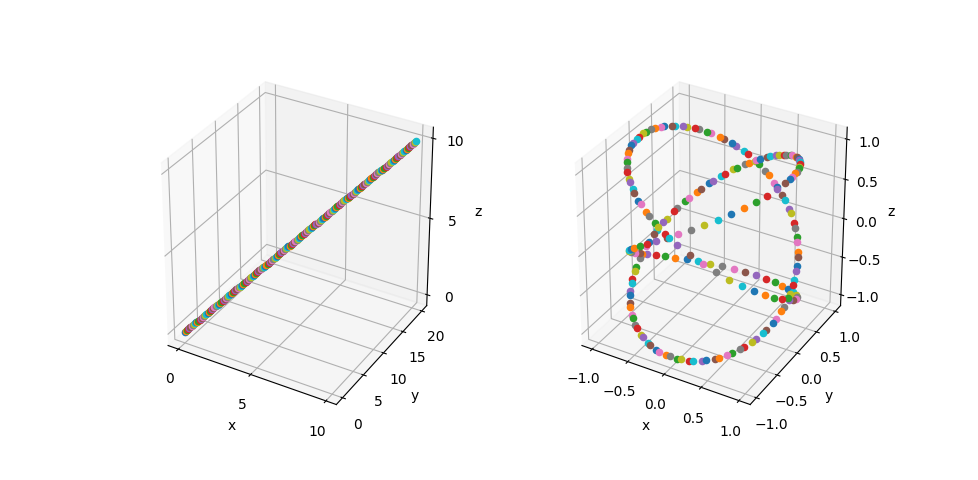
\includegraphics[width=0.8\textwidth]{images/transform.png}
\end{figure}



\begin{lstlisting}[language=python]
import numpy as np
from collections import namedtuple as nt
from infix import or_infix
from math import sin, cos, atan, tan, exp, log

Point = nt("Point", "x,y,z")

@or_infix
def vplus(point1, point2):
    x = point1.x + point2.x
    y = point1.y + point2.y
    z = point1.z + point2.z
    return Point(x, y, z)

@or_infix
def sprod(s, point):
    x = s * point.x
    y = s * point.y
    z = s * point.z
    return Point(x, y, z)

def Line(t):
    return Point(0, 0, 0) |vplus| ( t |sprod| Point(1, 2, 1) )

def transform(point):
    x = cos(point.x + point.y)
    y = sin(point.y + point.z)
    z = cos(point.z + point.x)
    return Point(x, y, z)

line = [Line(t) for t in np.arange(0.0, 10.0, 0.05)]
line2 = [transform(p) for p in line]
\end{lstlisting}